\documentclass{article}
\usepackage[a3paper,landscape,margin=8mm]{geometry}
\usepackage{tikz}
\usepackage{fontspec}
\setmainfont{Inter}
\pagestyle{empty}

\begin{document}
\noindent
\begin{center}
{\fontsize{13}{16}\selectfont\bfseries TheStreamDeck -- Front Panel Wireframes (70mm height)}\\[1pt]
{\fontsize{8}{10}\selectfont\color{gray} 92\% scale on A3 (actual case is 435 x 70mm). Multiply measurements by 1.087 for true dimensions.}
\end{center}
\vspace{2mm}

%% Scale: 0.92mm per mm (fits 435mm case on A3 landscape with 8mm margins)

%% ============================================================
%% OPTION A: Circular VU 45mm + 5" display + buttons + rotary
%% ============================================================

\noindent
{\fontsize{9}{11}\selectfont\bfseries A: 45mm circular VU + 5" display + 4 buttons + rotary}

\vspace{1mm}

\begin{center}
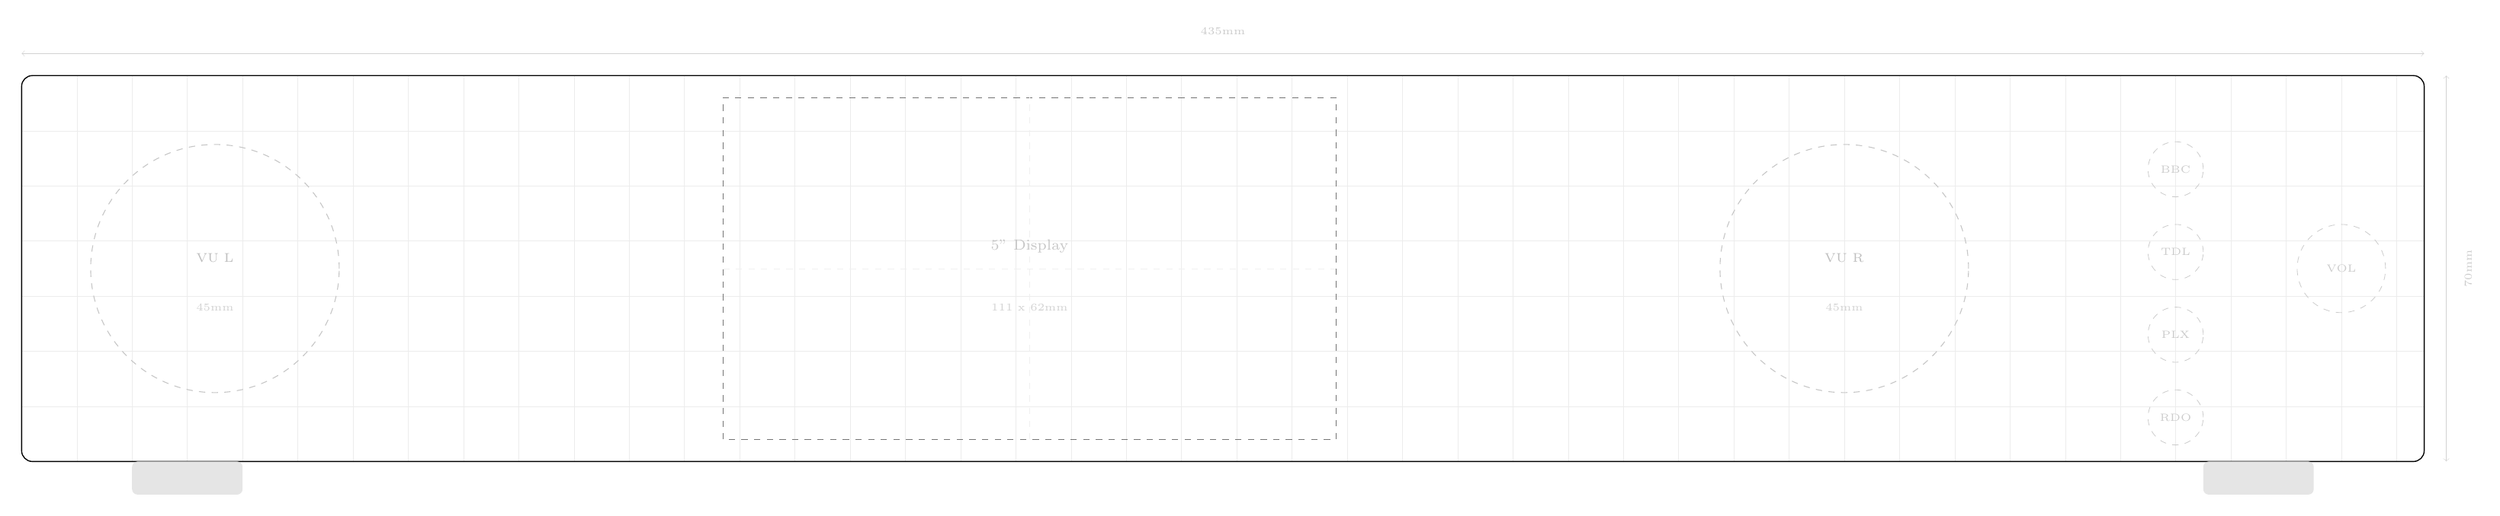
\begin{tikzpicture}[x=0.92mm, y=0.92mm]
  \def\cw{435} \def\ch{70}

  \begin{scope}
    \clip[rounded corners=1.8mm] (0,0) rectangle (\cw,\ch);
    \foreach \x in {0,10,...,435} { \draw[gray!15, line width=0.15pt] (\x,0) -- (\x,\ch); }
    \foreach \y in {0,10,...,70} { \draw[gray!15, line width=0.15pt] (0,\y) -- (\cw,\y); }
  \end{scope}
  \draw[black, line width=0.5pt, rounded corners=1.8mm] (0,0) rectangle (\cw,\ch);
  \fill[gray!20, rounded corners=0.9mm] (20,-6) rectangle (40,0);
  \fill[gray!20, rounded corners=0.9mm] (\cw-40,-6) rectangle (\cw-20,0);

  % VU L: 45mm circular
  \draw[gray!45, line width=0.4pt, dashed] (35,35) circle (22.5);
  \node[font=\fontsize{6}{8}\selectfont, text=gray!50] at (35,37) {VU L};
  \node[font=\fontsize{4}{5}\selectfont, text=gray!35] at (35,28) {45mm};

  % VU R: 45mm circular
  \draw[gray!45, line width=0.4pt, dashed] (330,35) circle (22.5);
  \node[font=\fontsize{6}{8}\selectfont, text=gray!50] at (330,37) {VU R};
  \node[font=\fontsize{4}{5}\selectfont, text=gray!35] at (330,28) {45mm};

  % 5" Display: 111 x 62mm centred between VUs
  \draw[black!55, line width=0.5pt, dashed] (127,4) rectangle (238,66);
  \node[font=\fontsize{7}{9}\selectfont, text=gray!45] at (182.5,39) {5" Display};
  \node[font=\fontsize{5}{7}\selectfont, text=gray!35] at (182.5,28) {111 x 62mm};
  \draw[gray!12, line width=0.2pt, dashed] (182.5,4) -- (182.5,66);
  \draw[gray!12, line width=0.2pt, dashed] (127,35) -- (238,35);

  % 4 buttons
  \foreach \i/\lbl in {1/BBC,2/TDL,3/PLX,4/RDO} {
    \pgfmathsetmacro{\bty}{70 - \i * 15 - 2}
    \draw[gray!40, line width=0.3pt, dashed] (390,\bty) circle (5);
    \node[font=\fontsize{3.5}{4}\selectfont, text=gray!40] at (390,\bty) {\lbl};
  }
  % Rotary
  \draw[gray!40, line width=0.3pt, dashed] (420,35) circle (8);
  \node[font=\fontsize{4}{5}\selectfont, text=gray!40] at (420,35) {VOL};

  % Dims
  \draw[gray!35, line width=0.2pt, <->] (0,\ch+4) -- (\cw,\ch+4);
  \node[font=\fontsize{5}{7}\selectfont, text=gray!40] at (\cw/2,\ch+8) {435mm};
  \draw[gray!35, line width=0.2pt, <->] (\cw+4,0) -- (\cw+4,\ch);
  \node[font=\fontsize{5}{7}\selectfont, text=gray!40, rotate=90] at (\cw+8,\ch/2) {70mm};
\end{tikzpicture}
\end{center}

\vspace{4mm}

%% ============================================================
%% OPTION B: Circular VU 50mm + 5" display + rotary only
%% ============================================================

\noindent
{\fontsize{9}{11}\selectfont\bfseries B: 50mm circular VU + 5" display + rotary only}

\vspace{1mm}

\begin{center}
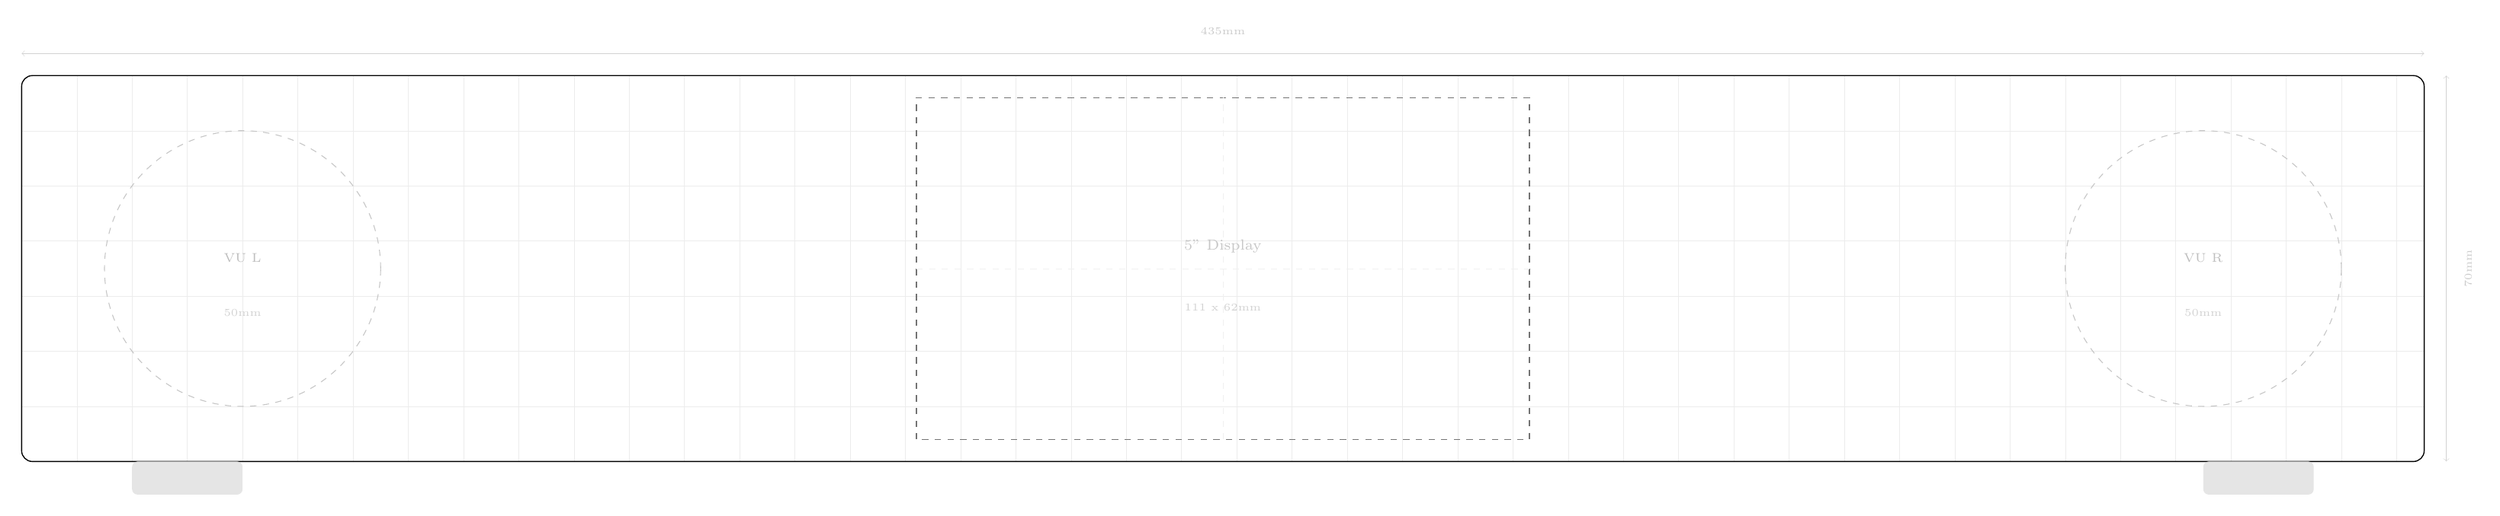
\begin{tikzpicture}[x=0.92mm, y=0.92mm]
  \def\cw{435} \def\ch{70}

  \begin{scope}
    \clip[rounded corners=1.8mm] (0,0) rectangle (\cw,\ch);
    \foreach \x in {0,10,...,435} { \draw[gray!15, line width=0.15pt] (\x,0) -- (\x,\ch); }
    \foreach \y in {0,10,...,70} { \draw[gray!15, line width=0.15pt] (0,\y) -- (\cw,\y); }
  \end{scope}
  \draw[black, line width=0.5pt, rounded corners=1.8mm] (0,0) rectangle (\cw,\ch);
  \fill[gray!20, rounded corners=0.9mm] (20,-6) rectangle (40,0);
  \fill[gray!20, rounded corners=0.9mm] (\cw-40,-6) rectangle (\cw-20,0);

  % VU L: 50mm circular
  \draw[gray!45, line width=0.4pt, dashed] (40,35) circle (25);
  \node[font=\fontsize{6}{8}\selectfont, text=gray!50] at (40,37) {VU L};
  \node[font=\fontsize{4}{5}\selectfont, text=gray!35] at (40,27) {50mm};

  % VU R: 50mm circular
  \draw[gray!45, line width=0.4pt, dashed] (395,35) circle (25);
  \node[font=\fontsize{6}{8}\selectfont, text=gray!50] at (395,37) {VU R};
  \node[font=\fontsize{4}{5}\selectfont, text=gray!35] at (395,27) {50mm};

  % 5" Display centred
  \draw[black!55, line width=0.5pt, dashed] (162,4) rectangle (273,66);
  \node[font=\fontsize{7}{9}\selectfont, text=gray!45] at (217.5,39) {5" Display};
  \node[font=\fontsize{5}{7}\selectfont, text=gray!35] at (217.5,28) {111 x 62mm};
  \draw[gray!12, line width=0.2pt, dashed] (217.5,4) -- (217.5,66);
  \draw[gray!12, line width=0.2pt, dashed] (162,35) -- (273,35);

  % Dims
  \draw[gray!35, line width=0.2pt, <->] (0,\ch+4) -- (\cw,\ch+4);
  \node[font=\fontsize{5}{7}\selectfont, text=gray!40] at (\cw/2,\ch+8) {435mm};
  \draw[gray!35, line width=0.2pt, <->] (\cw+4,0) -- (\cw+4,\ch);
  \node[font=\fontsize{5}{7}\selectfont, text=gray!40, rotate=90] at (\cw+8,\ch/2) {70mm};
\end{tikzpicture}
\end{center}

\vspace{4mm}

%% ============================================================
%% OPTION C: Rectangular VU 60x40mm (landscape) + 5" display + rotary
%% ============================================================

\noindent
{\fontsize{9}{11}\selectfont\bfseries C: 60x40mm rectangular VU (landscape) + 5" display + rotary}

\vspace{1mm}

\begin{center}
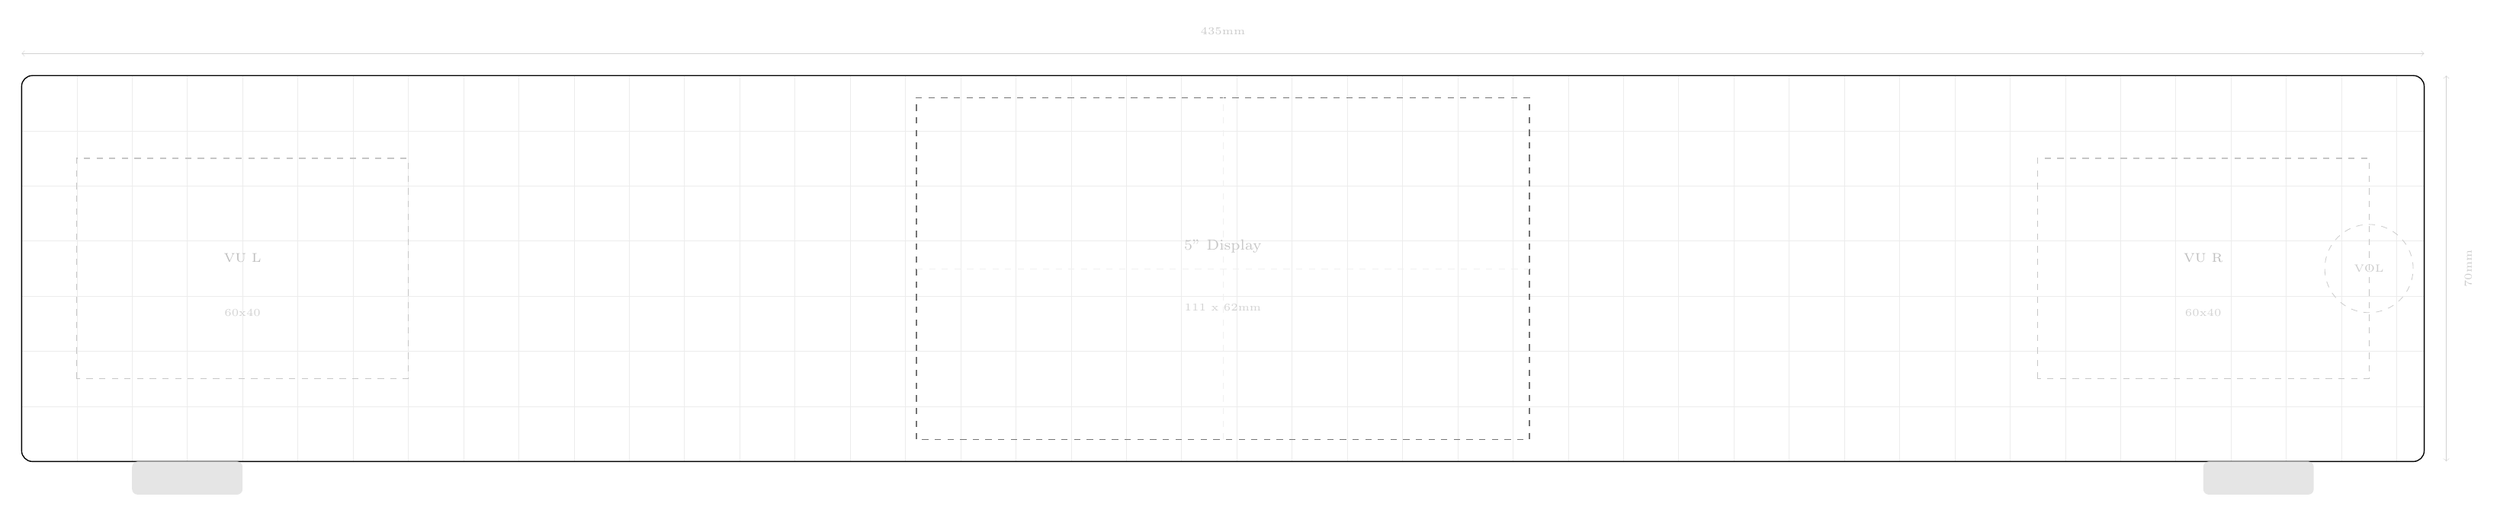
\begin{tikzpicture}[x=0.92mm, y=0.92mm]
  \def\cw{435} \def\ch{70}

  \begin{scope}
    \clip[rounded corners=1.8mm] (0,0) rectangle (\cw,\ch);
    \foreach \x in {0,10,...,435} { \draw[gray!15, line width=0.15pt] (\x,0) -- (\x,\ch); }
    \foreach \y in {0,10,...,70} { \draw[gray!15, line width=0.15pt] (0,\y) -- (\cw,\y); }
  \end{scope}
  \draw[black, line width=0.5pt, rounded corners=1.8mm] (0,0) rectangle (\cw,\ch);
  \fill[gray!20, rounded corners=0.9mm] (20,-6) rectangle (40,0);
  \fill[gray!20, rounded corners=0.9mm] (\cw-40,-6) rectangle (\cw-20,0);

  % VU L: 60x40mm landscape
  \draw[gray!45, line width=0.4pt, dashed] (10,15) rectangle (70,55);
  \node[font=\fontsize{6}{8}\selectfont, text=gray!50] at (40,37) {VU L};
  \node[font=\fontsize{4}{5}\selectfont, text=gray!35] at (40,27) {60x40};

  % VU R: 60x40mm landscape
  \draw[gray!45, line width=0.4pt, dashed] (365,15) rectangle (425,55);
  \node[font=\fontsize{6}{8}\selectfont, text=gray!50] at (395,37) {VU R};
  \node[font=\fontsize{4}{5}\selectfont, text=gray!35] at (395,27) {60x40};

  % 5" Display centred
  \draw[black!55, line width=0.5pt, dashed] (162,4) rectangle (273,66);
  \node[font=\fontsize{7}{9}\selectfont, text=gray!45] at (217.5,39) {5" Display};
  \node[font=\fontsize{5}{7}\selectfont, text=gray!35] at (217.5,28) {111 x 62mm};
  \draw[gray!12, line width=0.2pt, dashed] (217.5,4) -- (217.5,66);
  \draw[gray!12, line width=0.2pt, dashed] (162,35) -- (273,35);

  % Rotary
  \draw[gray!40, line width=0.3pt, dashed] (425,35) circle (8);
  \node[font=\fontsize{4}{5}\selectfont, text=gray!40] at (425,35) {VOL};

  % Dims
  \draw[gray!35, line width=0.2pt, <->] (0,\ch+4) -- (\cw,\ch+4);
  \node[font=\fontsize{5}{7}\selectfont, text=gray!40] at (\cw/2,\ch+8) {435mm};
  \draw[gray!35, line width=0.2pt, <->] (\cw+4,0) -- (\cw+4,\ch);
  \node[font=\fontsize{5}{7}\selectfont, text=gray!40, rotate=90] at (\cw+8,\ch/2) {70mm};
\end{tikzpicture}
\end{center}

\vspace{4mm}

%% ============================================================
%% OPTION D: Rectangular VU 50x60mm (portrait) + 5" display + buttons + rotary
%% ============================================================

\noindent
{\fontsize{9}{11}\selectfont\bfseries D: 50x60mm rectangular VU (portrait) + 5" display + 4 buttons + rotary}

\vspace{1mm}

\begin{center}
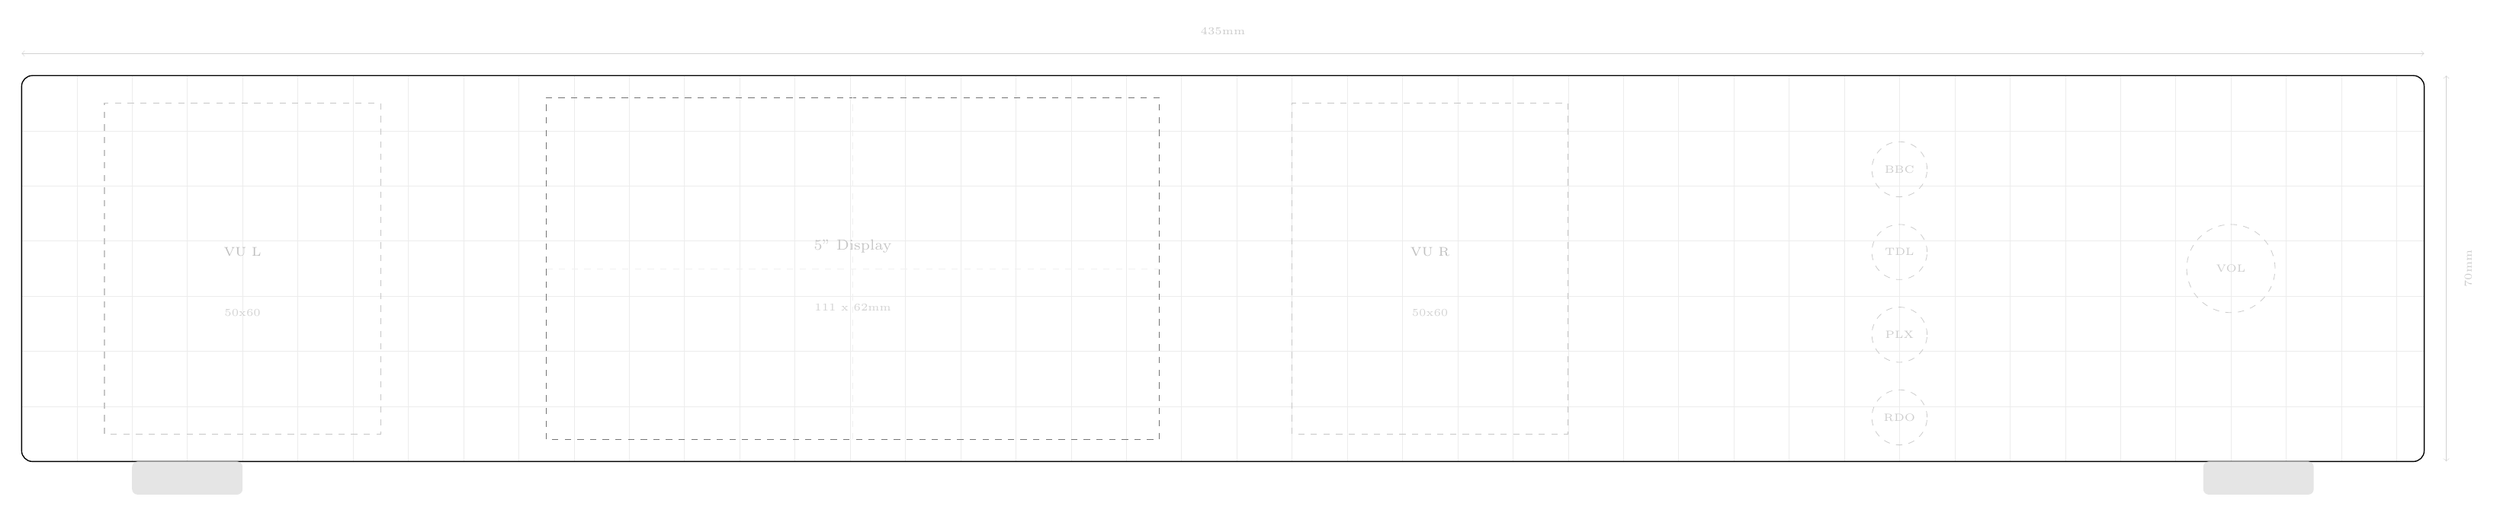
\begin{tikzpicture}[x=0.92mm, y=0.92mm]
  \def\cw{435} \def\ch{70}

  \begin{scope}
    \clip[rounded corners=1.8mm] (0,0) rectangle (\cw,\ch);
    \foreach \x in {0,10,...,435} { \draw[gray!15, line width=0.15pt] (\x,0) -- (\x,\ch); }
    \foreach \y in {0,10,...,70} { \draw[gray!15, line width=0.15pt] (0,\y) -- (\cw,\y); }
  \end{scope}
  \draw[black, line width=0.5pt, rounded corners=1.8mm] (0,0) rectangle (\cw,\ch);
  \fill[gray!20, rounded corners=0.9mm] (20,-6) rectangle (40,0);
  \fill[gray!20, rounded corners=0.9mm] (\cw-40,-6) rectangle (\cw-20,0);

  % VU L: 50x60mm portrait
  \draw[gray!45, line width=0.4pt, dashed] (15,5) rectangle (65,65);
  \node[font=\fontsize{6}{8}\selectfont, text=gray!50] at (40,38) {VU L};
  \node[font=\fontsize{4}{5}\selectfont, text=gray!35] at (40,27) {50x60};

  % 5" Display
  \draw[black!55, line width=0.5pt, dashed] (95,4) rectangle (206,66);
  \node[font=\fontsize{7}{9}\selectfont, text=gray!45] at (150.5,39) {5" Display};
  \node[font=\fontsize{5}{7}\selectfont, text=gray!35] at (150.5,28) {111 x 62mm};
  \draw[gray!12, line width=0.2pt, dashed] (150.5,4) -- (150.5,66);
  \draw[gray!12, line width=0.2pt, dashed] (95,35) -- (206,35);

  % VU R: 50x60mm portrait
  \draw[gray!45, line width=0.4pt, dashed] (230,5) rectangle (280,65);
  \node[font=\fontsize{6}{8}\selectfont, text=gray!50] at (255,38) {VU R};
  \node[font=\fontsize{4}{5}\selectfont, text=gray!35] at (255,27) {50x60};

  % Buttons
  \foreach \i/\lbl in {1/BBC,2/TDL,3/PLX,4/RDO} {
    \pgfmathsetmacro{\bty}{70 - \i * 15 - 2}
    \draw[gray!40, line width=0.3pt, dashed] (340,\bty) circle (5);
    \node[font=\fontsize{3.5}{4}\selectfont, text=gray!40] at (340,\bty) {\lbl};
  }
  % Rotary
  \draw[gray!40, line width=0.3pt, dashed] (400,35) circle (8);
  \node[font=\fontsize{4}{5}\selectfont, text=gray!40] at (400,35) {VOL};

  % Dims
  \draw[gray!35, line width=0.2pt, <->] (0,\ch+4) -- (\cw,\ch+4);
  \node[font=\fontsize{5}{7}\selectfont, text=gray!40] at (\cw/2,\ch+8) {435mm};
  \draw[gray!35, line width=0.2pt, <->] (\cw+4,0) -- (\cw+4,\ch);
  \node[font=\fontsize{5}{7}\selectfont, text=gray!40, rotate=90] at (\cw+8,\ch/2) {70mm};
\end{tikzpicture}
\end{center}

\vspace{3mm}

\begin{center}
{\fontsize{7}{9}\selectfont\color{gray}
\begin{tabular}{lcccc}
& \textbf{Case} & \textbf{Display} & \textbf{Physical VU} & \textbf{Controls} \\[2pt]
\textbf{A} & 435 $\times$ 70mm & 5" (111 $\times$ 62) & 2 $\times$ 45mm circular & 4 buttons + rotary \\
\textbf{B} & 435 $\times$ 70mm & 5" (111 $\times$ 62) & 2 $\times$ 50mm circular & rotary only \\
\textbf{C} & 435 $\times$ 70mm & 5" (111 $\times$ 62) & 2 $\times$ 60x40 rectangular & rotary only \\
\textbf{D} & 435 $\times$ 70mm & 5" (111 $\times$ 62) & 2 $\times$ 50x60 rect portrait & 4 buttons + rotary \\[3pt]
\hline \\[-6pt]
\multicolumn{5}{l}{\textit{Drawn at 92\% scale. NAD C 368: 435 $\times$ 102mm | NAD C 338: 435 $\times$ 70mm}}
\end{tabular}}
\end{center}

\end{document}
